% Copyright 2019
% IfV NRW, Fachhochschule Südwestfalen
% Arbeitsgebiet Mediengestaltung und Publishing
%
% Diese Datei wird eingesetzt für die Erstellung von Lerneinheiten im Verbundstudium.

% 2019-10-15
% Sandra Ciupka


\documentclass[paper=a4,fontsize=10pt,pagesize,headsepline=on,oneside,BCOR=13mm,
chapterprefix=false]{scrbook}
\setcounter{secnumdepth}{3}

%\title{}
%\author{}
%\date{\today}

\usepackage[ngerman]{babel}  % Trennung nach der neuen Rechtschreibung
\usepackage[T1]{fontenc}     % Trennung Umlaute
\usepackage[utf8]{inputenc}  % direkte Eingabe von Umlauten

\usepackage{lscape}
\usepackage{rotating}

\usepackage{color}
\usepackage{xcolor}
\graphicspath{{pics/}}

\usepackage{caption,graphicx}
\DeclareCaptionStyle{italic}
{labelfont={it,small},textfont={rm,it,small},justification=raggedright,position=bottom}
\captionsetup{labelfont={sf,bf},textfont={sf,bf},justification=raggedright,position=top}
\captionsetup[figure]{style=italic,width=1\textwidth}
\setcapwidth[]{1\textwidth}
\setcapmargin*{0pt}
\setcapindent{0em}

\usepackage{capt-of}  % für Bildbezeichner
\usepackage{sidecap}  % erlaubt \begin{wide} in figure
\usepackage{float}

\usepackage{tabularx}
\usepackage{tabulary}
\setlength\tymin{50pt}
\setlength\tymax{200pt}
\usepackage{etoolbox}
\apptocmd{\table}{\sffamily\small}{}{}
\usepackage{array,supertabular}
\setlength\extrarowheight{3pt}
\usepackage{multirow}
\usepackage{longtable}  % mehrseitige Tabellen ermöglichen
%\usepackage[table]{xcolor}

\newcommand\mpar[1]{\marginpar{\flushleft\sffamily\small #1}} % Marginalie
\usepackage{enumitem}
\usepackage{tcolorbox}

\usepackage{chngcntr} 
\counterwithout{footnote}{chapter}
\renewcommand\footnoterule{\vspace*{-3pt}%
\hrule width 107mm height 0.5pt \vspace*{5pt}}

\usepackage{scrextend}
% \deffootnote{<Markenbreite>}{<Absatzeinzug>}{<Definition>}
\deffootnote{2em}{0em}{\thefootnotemark\hspace{13.5pt}}
\renewcommand{\footnotesize}{\small}
\renewcommand*\thempfootnote{\arabic{mpfootnote}}
\footnotesep\baselineskip

\usepackage{fontspec}
\setmainfont[Ligatures=TeX]{Cambria}
\setsansfont[Ligatures=TeX]{Calibri}
\setmonofont[Scale=0.9]{Consolas}
\usepackage{setspace}   % Zeilenabstand
\usepackage{ragged2e}   % Flattersatz
\usepackage{microtype}  % optischer Randausgleich

\usepackage{listings}
\usepackage{amsthm}
\usepackage{calc}
\usepackage{fancyvrb}
\usepackage{framed}

\usepackage{geometry}
\geometry{lmargin=23.5mm,tmargin=29.4mm,rmargin=79.5mm,footskip=11mm,
	textwidth=107mm,textheight=243mm,headheight=8mm,
	headsep=12mm,marginparsep=5mm,marginparwidth=51mm%,showframe
}

% Klassisches BibTeX
%\usepackage[round]{natbib}
%\usepackage[fixlanguage]{babelbib}

% BibLaTeX
\usepackage[backend=biber,style=authoryear,natbib=true,hyperref=true]{biblatex}
%\addbibresource{Literatur.bib}
%\usepackage{csquotes}

% Formeln
%\usepackage[tbtags]{amsmath}
%\usepackage{amssymb} % Mathematische Symbole importieren
\usepackage{latexsym}
\usepackage{mathrsfs}
\usepackage{url} % bricht lange URLs "schön" um

%%%%%%%%%%%%%%%%%%%%%%%%%%%%%%%%%%%%%%%%%%%%%%%%%%%%%%%%%%%%%%%%%%%%%%%%%%%%%%%%%%%%%%%%%%%%%%%%%%%%%%%%%
%%%%%%%%%%%%%%%%%%%%%%%%%%%%%%%%%%%%%%%%%%%%%%%%%%%%%%%%%%%%%%%%%%%%%%%%%%%%%%%%%%%%%%%%%%%%%%%%%%%%%%%%%
% Ergänzung aus angelieferter Lerneinheit
\usepackage{textcomp}
\usepackage{here}
\usepackage{epstopdf}
%\usepackage[pdfencoding=auto,pdfborder={0 0 0}]{hyperref} % Lesezeichen im PDF
\usepackage{eurosym}
\usepackage{theorem}
\usepackage{amsmath,amssymb,dsfont}

\newcommand{\vtrans}{\begin{array}{c} \circ \\[-0.3cm]
		|    \\[-0.3cm]
		\bullet
\end{array} }

\setcounter{MaxMatrixCols}{20}

%%%%%%%%%%%%%%%%%%%%%%%%%%%%%%%%%%%%%%%%%%%%%%%%%%%%%%%%%%%%%%%%%%%%%%%%%%%%%%%%%%%%%%%%%%%%%%%%%%%%%%%%%
%%%%%%%%%%%%%%%%%%%%%%%%%%%%%%%%%%%%%%%%%%%%%%%%%%%%%%%%%%%%%%%%%%%%%%%%%%%%%%%%%%%%%%%%%%%%%%%%%%%%%%%%% 
% Kolumnenzeile
\usepackage{scrlayer-scrpage}

\clearpairofpagestyles

\automark*{section}
\ihead{\headmark}
\ohead{\pagemark} 


%%%%%%%%%%%%%%%%%%%%%%%%%%%%%%%%%%%%%%%%%%%%%%%%%%%%%%%%%%%%%%%%%%%%%%%%%%%%%%%%%%%%%%%%%%%%%%%%%%%%%%%%%

\setkomafont{pageheadfoot}{\small}
\setkomafont{pagehead}{\bfseries}

\renewcommand*{\chapterpagestyle}{scrheadings}
\addtokomafont{pagenumber}{\sffamily\bfseries} 					  % Anpassen der Schriftart der Seitenzahl
\setkomafont{pagehead}{\normalsize\normalfont\sffamily\bfseries}  % Setzen der Schriftart für Kopfzeile
\KOMAoptions{
	headwidth=(2\paperwidth-38mm+\textwidth)/3:0mm,
	headsepline=0.75pt
}
%\KOMAoptions{
	%footwidth=(2\paperwidth-30mm+\textwidth)/3:0mm % zentrierte Seitenzahl
%}
\ModifyLayer[addvoffset=.3ex]{scrheadings.head.below.line}

%%%%%%%%%%%%%%%%%%%%%%%%%%%%%%%%%%%%%%%%%%%%%%%%%%%%%%%%%%%%%%%%%%%%%%%%%%%%%%%%%%%%%%%%%%%%%%%%%%%%%%%%% 
% Hurenkinder, Schusterjungen

\clubpenalty = 10000
\widowpenalty = 10000
\displaywidowpenalty = 10000

%%%%%%%%%%%%%%%%%%%%%%%%%%%%%%%%%%%%%%%%%%%%%%%%%%%%%%%%%%%%%%%%%%%%%%%%%%%%%%%%%%%%%%%%%%%%%%%%%%%%%%%%% 
% Inhaltsverzeichnis

\usepackage{tocbasic}

\newcommand\textHGEcontentBold[1]{\sffamily\textbf{\large #1}}
\newcommand\textHGEcontent[1]{\sffamily\large #1}

\DeclareTOCStyleEntry[%
entryformat={\textHGEcontentBold},%
entrynumberformat={\textHGEcontentBold},%
pagenumberformat={\textHGEcontentBold},%
numwidth=21mm,%
linefill={\dotfill},%
beforeskip=21pt%
]{tocline}{chapter}

\DeclareTOCStyleEntry[%
entryformat={\textHGEcontent},%
entrynumberformat={\textHGEcontent},%
pagenumberformat={\textHGEcontent},%
numwidth=21mm,%
linefill={\dotfill},%
beforeskip=6pt,%
indent=0pt%
]{tocline}{section}

\DeclareTOCStyleEntry[%
entryformat={\textHGEcontent},%
entrynumberformat={\textHGEcontent},%
pagenumberformat={\textHGEcontent},%
numwidth=21mm,%
linefill={\dotfill},%
beforeskip=-1pt,%
indent=0pt%
]{tocline}{subsection}

\setcounter{tocdepth}{2}


%%%%%%%%%%%%%%%%%%%%%%%%%%%%%%%%%%%%%%%%%%%%%%%%%%%%%%%%%%%%%%%%%%%%%%%%%%%%%%%%%%%%%%%%%%%%%%%%%%%%%%%%%
% Überschriften

\RedeclareSectionCommand[beforeskip=0\baselineskip,
afterskip=1.0\baselineskip]{chapter}

\RedeclareSectionCommand[beforeskip=2.0\baselineskip,
afterskip=1.1\baselineskip]{section}

\RedeclareSectionCommand[beforeskip=2.0\baselineskip,
afterskip=1.1\baselineskip]{subsection}

\RedeclareSectionCommand[beforeskip=2.0\baselineskip,
afterskip=1.1\baselineskip]{subsubsection}

\RedeclareSectionCommand[beforeskip=1\baselineskip,
afterskip=1.3em]{paragraph}

\RedeclareSectionCommand[beforeskip=-0.5\baselineskip,
afterskip=-1em]{subparagraph}

%\usepackage{titlesec}
\setkomafont{chapter}{\large%\color{red}
}
\setkomafont{section}{\large%\color{blue}
}
\setkomafont{subsection}{\large%\color{green}
}
\setkomafont{subsubsection}{\large%\color{orange}
}

\makeatletter
\def\@seccntformat#1{\rlap{\csname the#1\endcsname}\hspace*{2.1cm}}
\def\chapterformat{\mbox{\rlap{\thechapter\autodot}\hspace*{1.9cm}\enskip}}
\def\sectionformat{\mbox{\rlap{\thesection\autodot}\hspace*{2.1cm}\enskip}}
\def\subsectionformat{\mbox{\rlap{\thesubsection\autodot}\hspace*{2.1cm}\enskip}}
\makeatother

%%%%%%%%%%%%%%%%%%%%%%%%%%%%%%%%%%%%%%%%%%%%%%%%%%%%%%%%%%%%%%%%%%%%%%%%%%%%%%%%%%%%%%%%%%%%%%%%%%%%%%%%% 
% Textgruppen
% Akzent

%\newenvironment{UMGEBUNGSNAME}[ANZAHL][OPTIONAL]{BEGIN}{END}
\newcommand\HF{\hrulefill\par}
\newsavebox{\ToDoBox}
\newenvironment{MyToDo}[1] %Name %Anzahl 
[] %OPTIONALEs Argument standardmäßig leer
{\vspace{12.5pt}%BEGIN
	\begin{lrbox}{\ToDoBox}%
		\begin{minipage}{\textwidth}
			% Fallunterscheidung 
			% -----------------------
			\newcommand{\TITEL}{\textbf{#1} 
					\hspace{0.5\textwidth} \par}
			\begin{addmargin}{1.5mm}
			\ifx&#1 % #1 is empty
			\else
			\TITEL  % #1 is nonempty
			\fi
			% -----------------------
			%\itshape 
		}%
		{%END
			\vspace{0.8ex}
			\end{addmargin}
		\end{minipage}
	\end{lrbox}%
	\colorbox{black!15}{\usebox{\ToDoBox}}
\vspace{5pt}}%

%%%%%%%%%%%%%%%%%%%%%%%%%%%%%%
% Spitzmarke

\newenvironment{Description}
{\begin{list}{}{\let\makelabel\Descriptionlabel
			\setlength\labelwidth{10pt}%
			\setlength\leftmargin{\labelwidth+\labelsep}}}%
		{\end{list}}
	\newcommand*\Descriptionlabel[1]{\bfseries{#1:}\hfil}
			
%%%%%%%%%%%%%%%%%%%%%%%%%%%%%%
% Eingezogene Textgruppen wie Definition, Satz usw.
\newenvironment{onequote}{\begin{list}{}{\leftmargin1.7em}\item[]}{\end{list}}
\newenvironment{twoquote}{\begin{list}{}{\leftmargin0em}\item[]}{\end{list}}
\newcommand{\quotepreskip}{~\\[-0.5cm]} 
\newcommand{\quoteheadersep}{\vspace{-1.7ex}}
\newcommand{\quotepostskip}{~\\[-0.3cm]} 

\newenvironment{Einzugit}[1]{\quotepreskip{\bfseries\sffamily #1}
	\quoteheadersep\begin{onequote}\itshape}{\end{onequote}\quotepostskip}

\newenvironment{Einzugup}[1]{\quotepreskip{\bfseries\sffamily #1}
	\quoteheadersep\begin{onequote}\upshape}{\end{onequote}\quotepostskip}

%%%%%%%%%%%%%%%%%%%%%%%%%%%%%%
% Nicht eingezogene Textgruppen mit Überschrift
\newenvironment{Textgruppe}[1]{\quotepreskip{\bfseries\sffamily #1}
	\quoteheadersep\begin{twoquote}\upshape}{\end{twoquote}\quotepostskip}

%%%%%%%%%%%%%%%%%%%%%%%%%%%%%%
% Baustelle – für spätere Verwendung

%\newtheoremstyle{break}	%
%{9pt}{9pt}					% Abstand oben und unten
%{\raggedright}%
%{-12pt} 					% Überschrift: Einzug
%{\sffamily\bfseries}{:} 	% Font und Satzzeichen danach
%{\newline} 				% Abstand nach Überschrift
%{}							% Überschriftenspezifikation
%\theoremstyle{break}

%%%%%%%%%%%%%%%%%%%%%%%%%%%%%%%%%%%%%%%%%%%%%%%%%%%%%%%%%%%%%%%%%%%%%%%%%%%%%%%%%%%%%%%%%%%%%%%%%%%%%%%%%
%%%%%%%%%%%%%%%%%%%%%%%%%%%%%%%%%%%%%%%%%%%%%%%%%%%%%%%%%%%%%%%%%%%%%%%%%%%%%%%%%%%%%%%%%%%%%%%%%%%%%%%%% 
% Jetzt beginnt das eigentliche Dokument

\begin{document}

	\newgeometry{rmargin=23.5mm,tmargin=29.4mm,textwidth=163mm,textheight=243mm,headheight=8mm}
	
	%\maketitle
	
	\pagestyle{headings}
	\tableofcontents
			
	\restoregeometry
	
	\raggedbottom  % kein einheitlicher Rand unten (-> schönere Abstände zwischen Absätzen)
	\RaggedRight   % Flattersatz mit Trennungen
	
	\begin{spacing}{1.1} % Zeilenabstand
		
		% Copyright 2019
% IfV NRW, Fachhochschule Südwestfalen
% Arbeitsgebiet Mediengestaltung und Publishing
%
% Diese Datei wird eingesetzt für die Erstellung von Lerneinheiten im Verbundstudium.

% 2019-10-15
% Sandra Ciupka


\chapter{Überschrift Vorwort}

Lorem ipsum dolor sit amet, consetetur sadipscing elitr, sed diam nonumy eirmod tempor invidunt ut labore et dolore magna aliquyam erat, sed diam voluptua. At vero eos et accusam et justo duo dolores et ea rebum. Stet clita kasd gubergren, no sea takimata sanctus est Lorem ipsum dolor sit amet. Lorem ipsum dolor sit amet, consetetur sadipscing elitr, sed diam nonumy eirmod tempor invidunt ut labore et dolore magna aliquyam erat, sed diam voluptua. At vero eos et accusam et justo duo dolores et ea rebum. Stet clita kasd gubergren, no sea takimata sanctus est Lorem ipsum dolor sit amet.
\bigskip





	
		% Copyright 2019
% IfV NRW, Fachhochschule Südwestfalen
% Arbeitsgebiet Mediengestaltung und Publishing
%
% Diese Datei wird eingesetzt für die Erstellung von Lerneinheiten im Verbundstudium.

% 2019-10-15
% Sandra Ciupka


\chapter{Überschrift Textebene-1}

Lorem ipsum dolor sit amet, consetetur sadipscing elitr, sed diam nonumy eirmod tempor invidunt ut labore et dolore magna aliquyam erat, sed diam voluptua. At vero eos et accusam et justo duo dolores et ea rebum. Stet clita kasd gubergren, no sea takimata sanctus est Lorem ipsum dolor sit amet. Lorem ipsum dolor sit amet, consetetur sadipscing elitr, sed diam nonumy eirmod tempor invidunt ut labore et dolore magna aliquyam erat, sed diam voluptua. At vero eos et accusam et justo duo dolores et ea rebum. Stet clita kasd gubergren, no sea takimata sanctus est Lorem ipsum dolor sit amet.
\bigskip

Lorem ipsum dolor sit amet, consetetur sadipscing elitr, sed diam nonumy eirmod tempor invidunt ut labore et dolore magna aliquyam erat, sed diam voluptua. At vero eos et accusam et justo duo dolores et ea rebum. Stet clita kasd gubergren, no sea takimata sanctus est Lorem ipsum dolor sit amet. Lorem ipsum dolor sit amet, consetetur sadipscing elitr, sed diam nonumy eirmod tempor invidunt ut labore et dolore magna aliquyam erat, sed diam voluptua. At vero eos et accusam et justo duo dolores et ea rebum. Stet clita kasd gubergren, no sea takimata sanctus est Lorem ipsum dolor sit amet.

%%%%%%%%%%%%%%%%%%%%%%%%%%%%%%%%%%%%%%%%%%%%%%%%%%%%%%%%%%%%%%%%%%%%%%%%%%%%%%%%%%%%%%%%%%%%%%%%%%%%%%%%%%%
\section{Überschrift Textebene-2}

Lorem ipsum dolor sit amet, consetetur sadipscing elitr, sed diam nonumy eirmod tempor invidunt ut labore et dolore magna aliquyam erat, sed diam voluptua. At vero eos et accusam et justo duo dolores et ea rebum. Stet clita kasd gubergren, no sea takimata sanctus est Lorem ipsum dolor sit amet. Lorem ipsum dolor sit amet, consetetur sadipscing elitr, sed diam nonumy eirmod tempor invidunt ut labore et dolore magna aliquyam erat, sed diam voluptua. At vero eos et accusam et justo duo dolores et ea rebum. Stet clita kasd gubergren, no sea takimata sanctus est Lorem ipsum dolor sit amet.

% Abbildung: 107 mm
\begin{figure}[!h]
	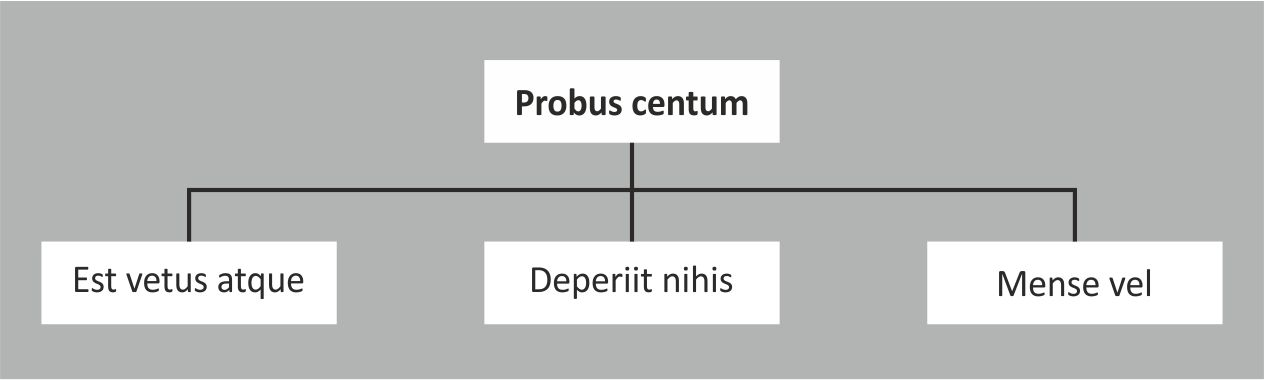
\includegraphics[width=10.7cm]{pics/Abb-001.jpg}
	\caption{Beschriftung einer Abbildung}
	\label{Abb-001}
\end{figure}

%%%%%%%%%%%%%%%%%%%%%%%%%%%%%%%%%%%%%%%%%%%%%%%%%%%%%%%%%%%%%%%%%%%%%%%%%%%%%%%%%%%%%%%%%%%%%%%%%%%%%%%%%%%
\subsection{Überschrift Textebene-3}

Lorem ipsum dolor sit amet, consetetur sadipscing elitr, sed diam nonumy eirmod tempor invidunt ut labore et dolore magna aliquyam erat, sed diam voluptua. At vero eos et accusam et justo duo dolores et ea rebum. Stet clita kasd gubergren, no sea takimata sanctus est Lorem ipsum dolor sit amet. Lorem ipsum dolor sit amet, consetetur sadipscing elitr, sed diam nonumy eirmod tempor invidunt ut labore et dolore magna aliquyam erat, sed diam voluptua. At vero eos et accusam et justo duo dolores et ea rebum. Stet clita kasd gubergren, no sea takimata sanctus est Lorem ipsum dolor sit amet.

% Tabelle mit flexiblen Spalten
\begin{table}
	\captionabove{Beschriftung einer Tabelle}
	\begin{tabulary}{10.7cm}{|L|L|L|L|L|L|} % linksbündig
		\hline
		Zelle 1 & 2	& 3 & Zelle 4 & 5 & 6\\
		\hline
		Zelle 7	& 8	& 9 & Zelle 10 & 11 & 12\\
		\hline
	\end{tabulary}
\end{table}








		
	\end{spacing}

%%%%%%%%%%%%%%%%%%%%%%%%%%%%%%%%%%%%%%%%%%%%%%%%%%%%%%%%%%%%%%%%%%%%%%%%%%%%%%%%%%%%%%%%%%%%%%%%%%%%%%%%%
% Abbildungsverzeichnis
% Tabellenverzeichnis

	\listoftables
	\addcontentsline{toc}{section}{Tabellenverzeichnis}
	\listoffigures
	\addcontentsline{toc}{section}{Abbildungsverzeichnis}

%%%%%%%%%%%%%%%%%%%%%%%%%%%%%%%%%%%%%%%%%%%%%%%%%%%%%%%%%%%%%%%%%%%%%%%%%%%%%%%%%%%%%%%%%%%%%%%%%%%%%%%%%
% Klassisches BibTeX

	%\nocite{*}
	%\bibliographystyle{babplain}
	%\bibliographystyle{alphadin} 	% Festlegung Art Zitierung (Havardmethode: Abkuerzung Autor+Jahr)
	
	%Literaturliste soll im Inhaltsverzeichnis auftauchen:
	%\newpage
	%\addcontentsline{toc}{section}{Literaturverzeichnis}
	%\bibliography{Literatur.bib}   % Datei aus Citavi
	
%%%%%%%%%%%%%%%%%%%%%%%%%%%%%%%%%%%%%%%%%%%%%%%%%%%%%%%%%%%%%%%%%%%%%%%%%%%%%%%%%%%%%%%%%%%%%%%%%%%%%%%%% 
% BibLaTeX

	\nocite{*}

	%\newpage
	%\ifkomabibtotocnumbered{true}
	% Copyright 2019
% IfV NRW, Fachhochschule Südwestfalen
% Arbeitsgebiet Mediengestaltung und Publishing
%
% Diese Datei wird eingesetzt für die Erstellung von Lerneinheiten im Verbundstudium.

% 2019-10-15
% Sandra Ciupka


\begin{thebibliography}{}
	\bibitem{Kurzform} Vorname Nachname, Titel, Verlag (Jahr).
\end{thebibliography}


    % Ergänzung angelieferter Daten
	\addcontentsline{toc}{section}{Literaturverzeichnis}
	%\renewcommand\chaptername{\protect Literaturverzeichnis}
	%\printbibliography
	
\end{document}